\documentclass[../main.tex]{subfiles}
%!TEX root = ./appendixLinearActuator.tex
\graphicspath {{../}}

\begin{document}
\subsection{Linear Actuator} 
\label{linearActuator}
\begin{figure}[H]
	\centering
	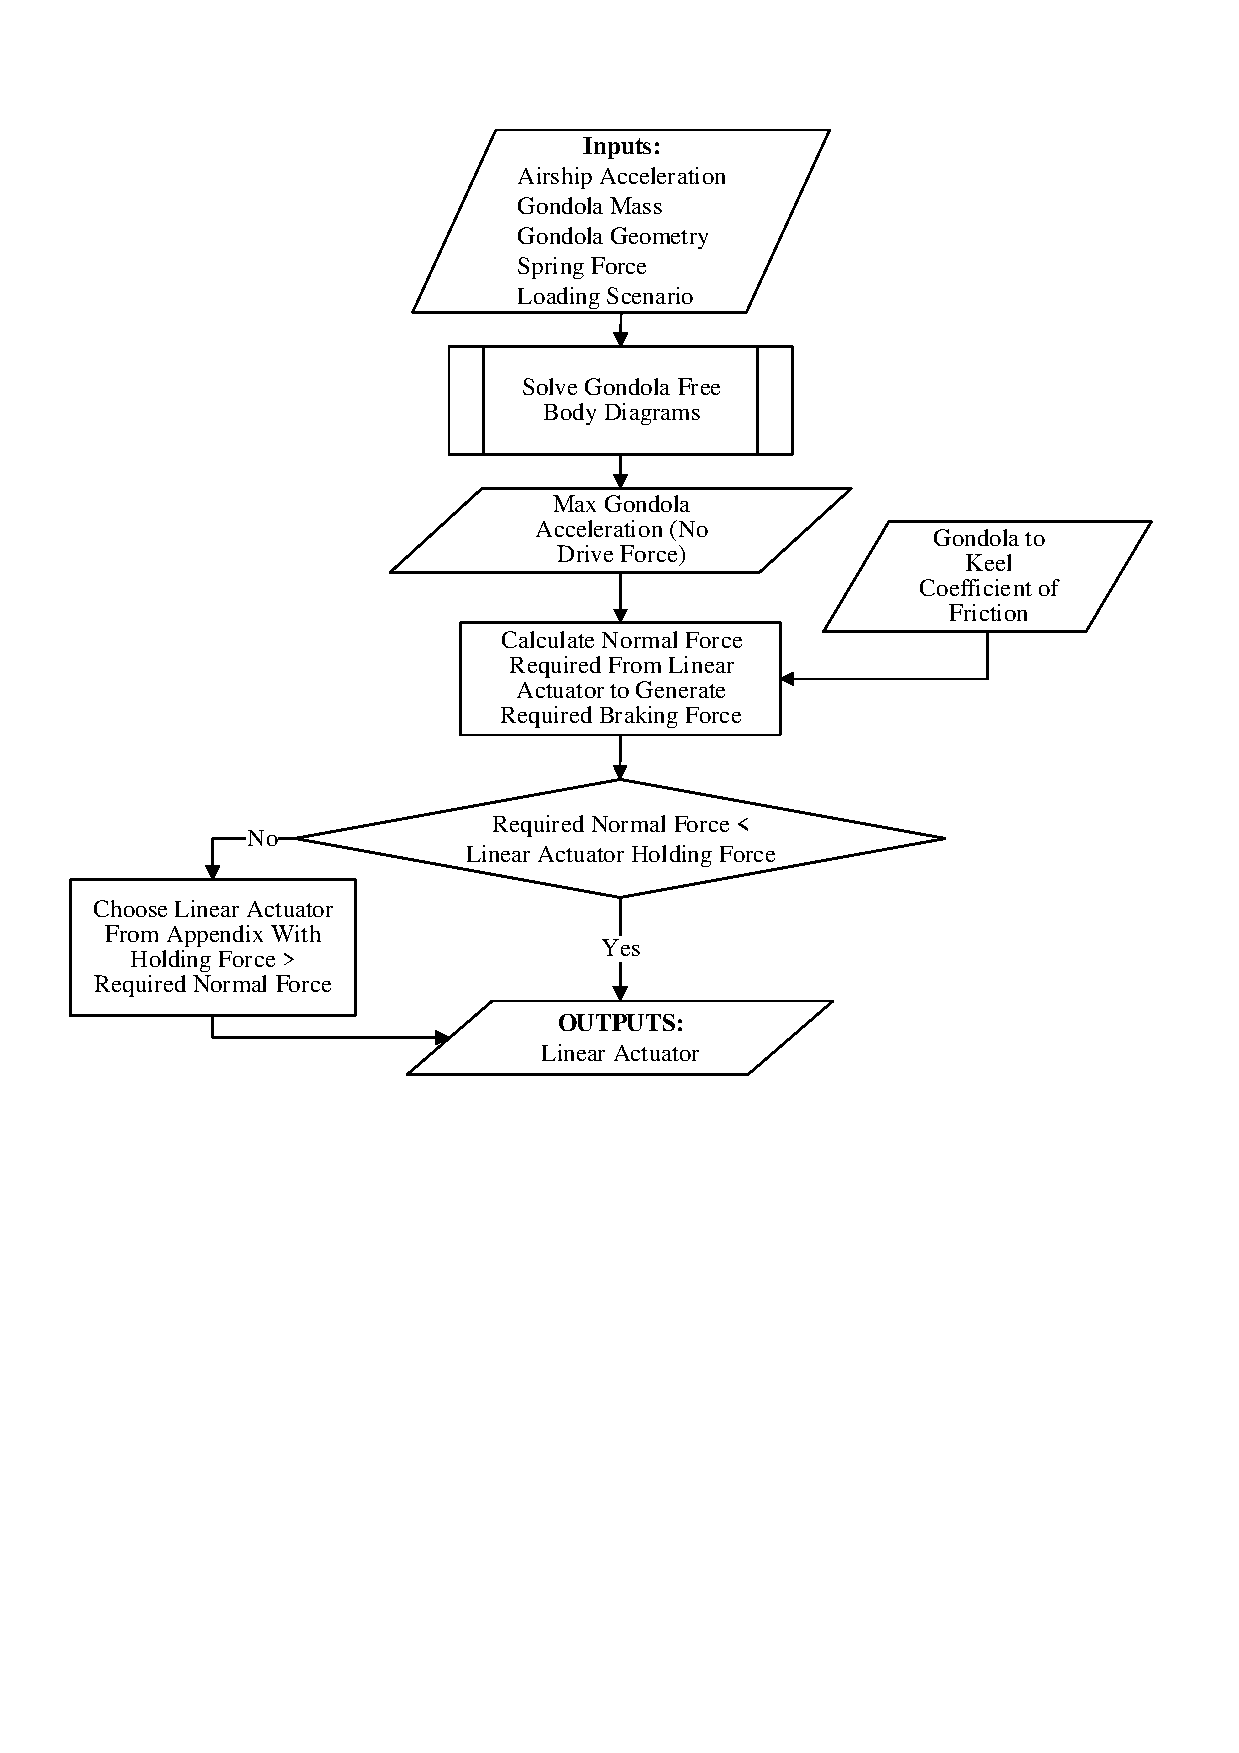
\includegraphics[width=\linewidth]{img/paramaterization/linearActuator.pdf}
	\caption{Parametrization Outline for the Linear Actuator}
	\label{fig:linearActuatorParametrization}
\end{figure}

The linear actuator analysis is preformed to ensure that the holding force of the linear actuator generates a great enough friction to keep the gondola from moving. The analysis first solves for the acceleration in a scenario similar to that of worst case scenario explained in System Modelling section \ref{loadingScenarios}, Maximum Downward Force, and Figure \ref{fig:scenario1} and in friction wheel slip section \ref{frictionSlip}, the only difference is that the friction wheel motor will not be powered, therefore the drive force $F_{Drive} = 0$. The free-body diagram for this case can be seen below in Figure \ref{fig:sideGondolaNoDrive}.

\begin{figure}[H]
	\centering
	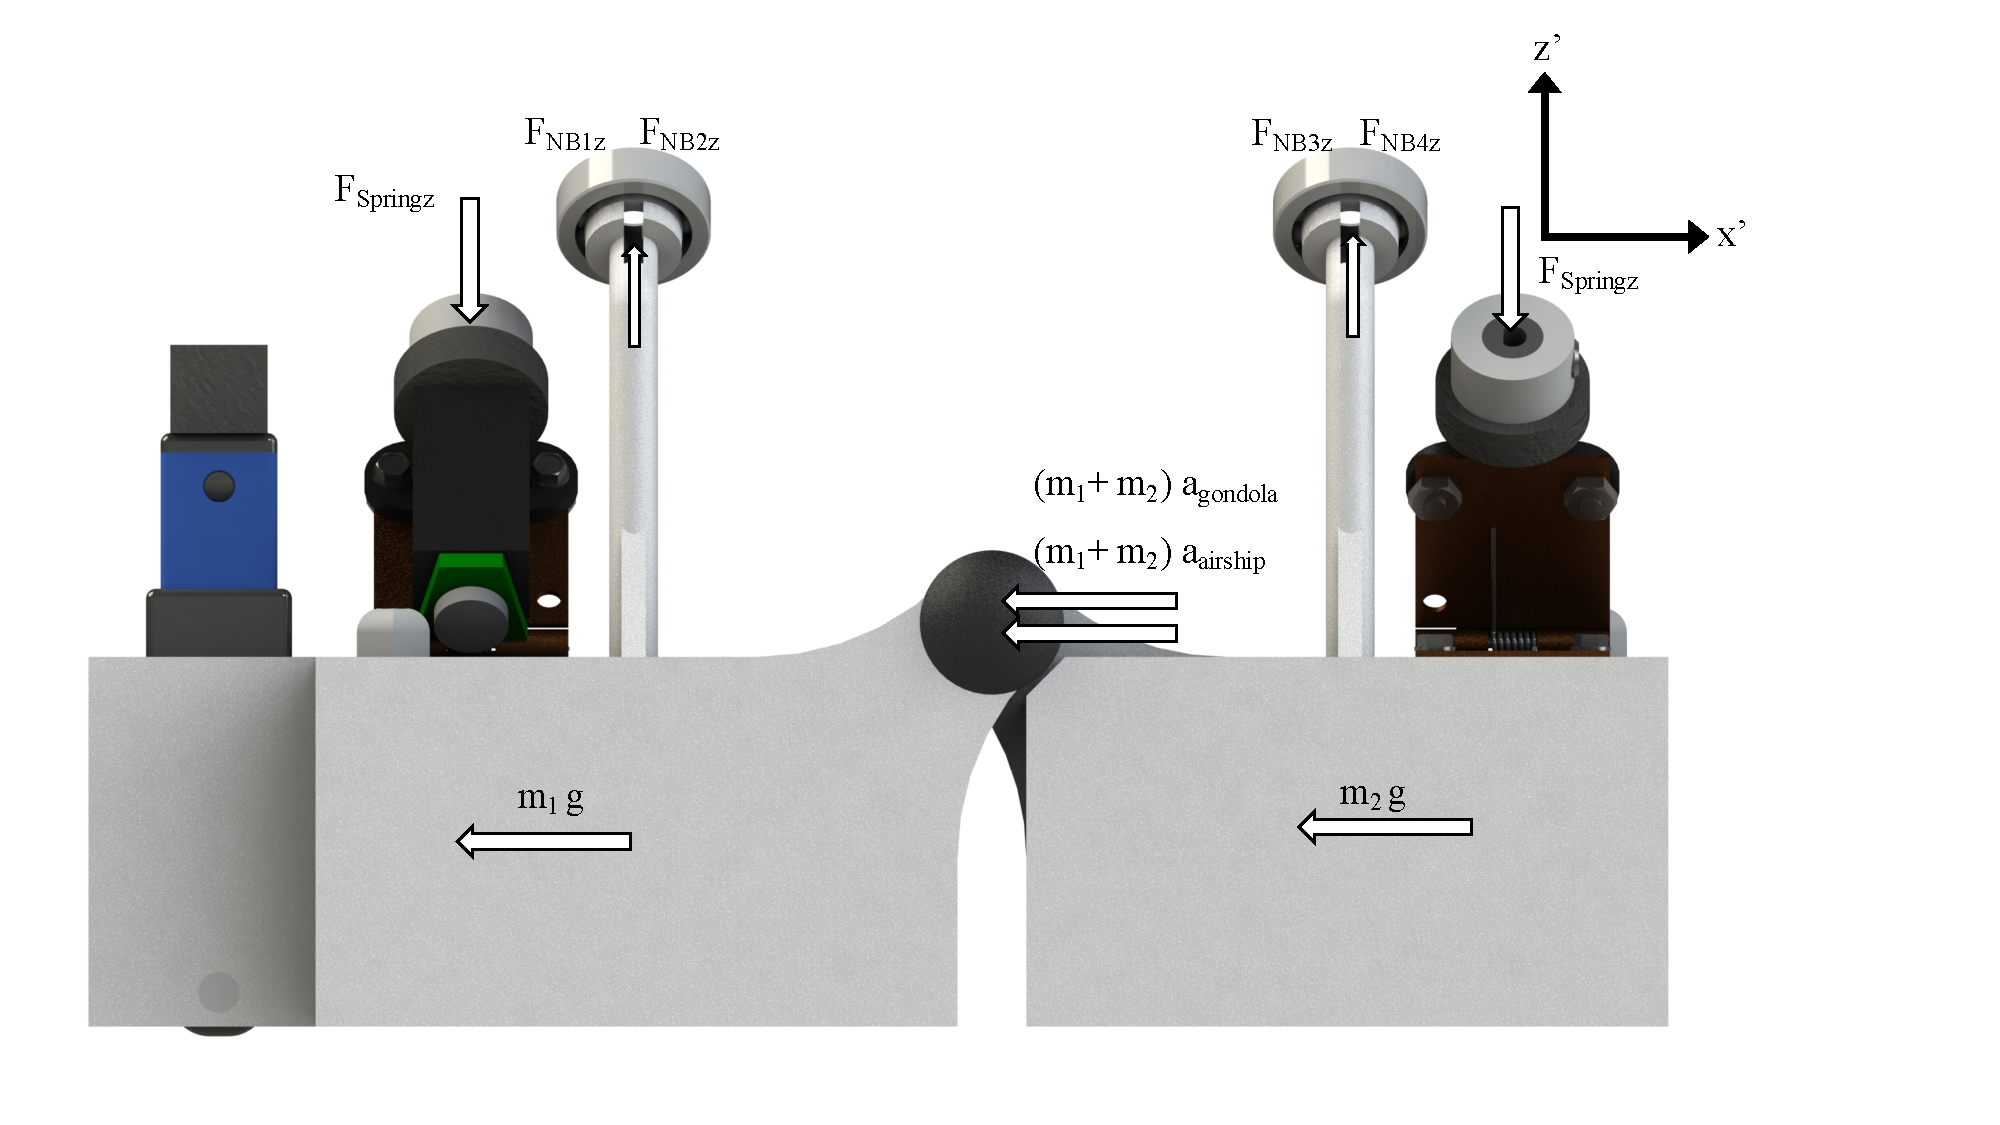
\includegraphics[width=1.1\textwidth]{img/gondola/sideGondolaNoDrive.pdf}
	\caption{Side View of Gondola With Maximum Downward Force and No Drive Force}
	\label{fig:sideGondolaNoDrive}
\end{figure}

The inputs required to run this analysis are the geometry of the friction wheel, the motor, the hinge, the gondola, as well as the material properties of the braking surface, the mass of each gondola section, the maximum achievable thruster acceleration and the loading conditions specific to the worst case scenario. The sum of forces used to solve for the case are as follows. 
\begin{equation} \label{FxGondLA}
\Sigma F_{x} : (m_{1}+m_{2}) a_{gondola} + F_{NB3_{x}} + F_{NB4_{x}} = \sin(\phi) (m_{1} + m_2)g + \cos(\beta) (m_1+m_2) a_{Thrust} 
\end{equation}
\begin{equation} \label{FyGondLA}
\hspace{12pt}\Sigma F_{y} : F_{NB1_{y}} - F_{NB2_{y}} - F_{NB3_{y}} + F_{NB4_{y}} =  F_{Springy} -F_{Springy} 
\end{equation}
\begin{multline} \label{FzGondLA}
\Sigma F_{z} : F_{NB1_{z}} + F_{NB2_{z}} + F_{NB3_{z}} + F_{NB4_{z}} =\\ \cos(\phi) (m_{1} + m_2)g -  F_{Springz} - F_{Springz} + \sin(\beta) (m_1+m_2) a_{Thrust}
\end{multline}
The spring forces $F_{Springz}$ and $F_{Springy}$ are acting on the keel at 45\textdegree. The following equation can be used to define the spring forces. 
\begin{equation}
F_{Springz} = F_{Springy} = \frac{\sqrt{2}}{2} F_{Spring}
\end{equation} \\

The holding force $F_{brake}$ must then be greater than the calculated acceleration $a_{gondola}$. The holding force is dependent on the friction force between the polyurethane and rubber contact piece of the linear actuator, as seen in Figure \ref{fig:linearActuatorAndMotor}.  The holding force is related to the linear actuator for $F_{LA}$ by the equation \ref{eqn:brake} below.
\begin{equation}
\label{eqn:brake}
F_{brake} = \mu_{braking surface} F_{LA}
\end{equation}

The value for $\mu_{braking surface}$ is based on the coefficient of friction between rubber and polyurethane which is 0.65 \cite{Friction}. Once the required linear actuator force is calculated it is compared with the Actuonix linear actuator datasheet can be found in Appendix \ref{LinAct} in order to make sure that the force is achievable.\\

As explained above the analysis first solves for the acceleration of the gondola, while the motors are not driving, with the inputs specified in the System Modelling section \ref{sampleCalcs} Sample Calculation Conditions, the acceleration was 5.35[$\dfrac{m}{s^2}$]. Therefore the required holding force is simply the acceleration multiplied by the mass of the airship, which is 11.68[N]. The required linear actuator force to hold the gondola is calculated in the following equation:
\begin{equation}
\label{eqn:brake}
F_{LA} = \frac{F_{brake}}{\mu_{braking surface} } = \frac{11.68[N]}{0.65} = 17.96
\end{equation}
The linear actuator datasheet from Actuonix in Appendix \ref{LinAct} with 22N holding force was chosen. 
\end{document}